\section{Modo Real}

\subsection{Introducción}

Por una cuestión de compatibilidad hacia atrás, al inicializar un procesador Intel, el mismo funciona como un 8086, lo que conocemos como \texttt{Modo Real}. En este modo, no existe la protección por hardware, es decir, cualquier código en ejecución tiene acceso a todos los segmentos de memoria y puede utilizar cualquier instrucción del 8086. Para poder utilizar otras instrucciones y funcionalidades mas avanzadas, también habilitando la protección por hardware, se debe pasar a Modo Protegido.

\subsection{A20}
El addressing line \texttt{A20} forma parte del bus de direcciones del procesador. En un \texttt{8086}, este bus tiene 20 lineas, numeradas de la 0 a la 19. Sin embargo, cuando salio al mercado el \texttt{80286}, el primero en soportar el modo protegido,  el bus de direcciones paso a tener 24 bits. El problema que surgió es que muchos programadores en su código del \texttt{8086} utilizaban lo que se conoce como wrap-around. Es decir, cuando accedían a memoria, utilizaban el overflow en el bus de direcciones como parte de la lógica de sus programas. El 80286 no soportaba este overflow, rompiendo la compatibilidad hacia atrás, dado que tenia 4 lineas de address adicionales.

Para solucionar este problema, a IBM se le ocurrió utilizar un pin del controlador del teclado que estaba sin usar y conectarlo a la linea 20 del bus de direcciones para poder forzar el overflow en los programas viejos. Por esta razón, antes de pasar a modo protegido se debe habilitar esta linea, para poder utilizar todo el espacio direccionable por todas las lineas del bus de direcciones. Esto se realiza a través de un handshake que consiste en enviar una sequencia de bytes particular por la linea de teclado.

\subsection{Global Descriptor Table}

Antes de poder pasar a modo protegido, debemos configurar de GDT. La GDT es un arreglo en memoria de hasta 8192 entradas de 8 bytes cada una, cada una de estas entradas define la configuración de un segmento de memoria, o de una tarea. En nuestro código, puede encontrarse en \texttt{gdt.h} la estructura de \texttt{gdt\_entry} con sus respectivos parámetros de configuración. La figura de aquí abajo muestra el significado de los campos para un descriptor de segmento.

\begin{figure}[h!]
  \centering
    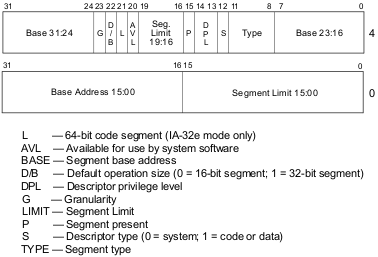
\includegraphics[width=0.5\textwidth]{images/segment_descriptor}
  \caption{Segment Descriptor}
\end{figure}

En su primera encarnación, la GDT nos permite configurar permisos de acceso a la memoria, utilizando el conocido modelo de memoria segmentado. En nuestro caso particular, nosotros hacemos un identity mapping de los primeros 500 MB de memoria (que por otro lado es más de lo que utilizamos), evitando de esta forma tener que realmente tener en cuenta los efectos de segmentación. En concreto, el hacer un identity mapping nos permite "deshabilitar" la segmentación: a pesar de que no sea posible a nivel procesador desactivarla, y el proceso de traslación de direcciones se realiza igual, no tenemos efectos colaterales. Más adelante se extendió la capacidad de la GDT para soportar el entorno multitarea que conocemos hoy en día, pero trataremos sobre ese tema más adelante.

Para nuestro kernel habilitamos un total de 5 segmentos de memoria fuera del NULL segment y los 8 reservados por la cátedra. Los 5 segmentos corresponden a, respectivamente: código y datos con nivel de protección 0, código y datos con nivel de protección 3, y video con protección 0. Como dijimos antes, los 4 segmentos que no corresponden a vídeo están mapeados sobre el mismo espacio de memoria, cambiando únicamente el nivel de privilegio requerido para acceder. Esta elección permite que el esquema de memoria no cambie a lo largo del código, ayudando a la comprensión y correctitud del código. En tanto al segmento para video, este mapea las direcciones específicas del frame buffer, y le damos acceso sólo a nivel 0, pudiendo así evitar que las tareas del usuario cambien los datos de video.

Luego de haber configurado la GDT, la instrucción \command{lgdt} nos permite cargar un descriptor de GDT indicando la ubicación de la GDT en la memoria para que el procesador pueda comenzar a aplicar segmentación como corresponde. Este descriptor contiene la dirección física de la GDT, así como el tamaño de la estructura. Cabe destacar que el espacio reservado para la GDT es de 32 entradas: 5 correspondientes a las del kernel, 1 del NULL descriptor, 8 reservadas por la cátedra, y el resto destinadas al manejo de tareas.

\subsection{Pasaje a Modo Protegido}

Una vez armada la GDT y habilitado la puerta A20, debemos habilitar Modo Protegido. El modo de protección esta definido por el bit menos significativo del registro \reg{CR0}. Usando un OR con \addr{0x1}, habilitamos este bit.

Una vez que tenemos todas las estructuras necesarias armadas, hay que hacer un \command{jmp far} al segmento de código de nivel 0 en la \texttt{GDT}. De esta forma finalmente habilitamos la protección por hardware y pasamos a Modo Protegido. A partir de aquí es fundamental poner los selectores de segmentos correspondientes a los datos y video, habilitándonos efectivamente para el uso de memoria y el frame buffer. Cabe destacar, además, que no necesariamente tenemos una pila que podamos utilizar, por lo que es importante poner los registros correspondientes en valores que nos sean útiles.